\documentclass[11pt,a4paper]{article}
\usepackage{a4wide}
\usepackage[utf8]{inputenc}
\usepackage[T2A]{fontenc}
\usepackage{graphics,graphicx,epsfig}
\usepackage{amssymb,amsfonts,amsthm,amsmath,mathtext,cite,enumerate,float}
\usepackage[english,russian]{babel}
\usepackage[all]{xy}
\usepackage{morefloats}
\usepackage{pgf}
\usepackage[debug,outputdir={docgraphs/}]{dot2texi}
\usepackage{tikz}
\usepackage{scalefnt}
\usepackage{listings}
\usepackage{float}
\usepackage{verbatim}
\usepackage{placeins}
\usepackage{url}
\usepackage{babelbib}
\usepackage{pbox}
\usepackage{grffile}
\usepackage{color}
\usepackage{xfrac}
\usepackage{comment}
\usepackage{rotating}
\usepackage{slashbox}
\usepackage{caption}
\usepackage{subcaption}

\makeatletter
\def\@settitle{\begin{center}%
    \baselineskip14\p@\relax
    \bfseries
    \@title
  \end{center}%
}

\makeatother

\newcommand{\bomega}{\boldsymbol{\omega}}

\begin{document}

\begin{center}
  МОДИФИКАЦИЯ ФУНКЦИОНАЛА ОШИБКИ В ЗАДАЧАХ НЕЛИНЕЙНОЙ РЕГРЕССИИ ДЛЯ УЧЕТА ПОГРЕШНОСТИ В ИЗМЕРЯЕМЫХ ДАННЫХ

  \bigskip
  Г.\,И.~Рудой
\end{center}

\section{Введение}

В ряде экспериментальных приложений возникает задача нахождения оптимальных
коэффициентов $\boldsymbol{\omega}$ некоторой регрессионной модели $f$, представленной в
виде аналитической формулы, по набору экспериментальных данных. Для этого
в предположении о нормальном распределении регрессионных остатков
строится функционал, являющийся суммой квадратов отклонений экспериментальных
точек $y_i$ от регрессионной кривой: $\sum_i (y_i - f(x_i, \boldsymbol{\omega}))^2$.
Для численного решения этой задачи широко применяется алгоритм Левенберга-Марквардта
\cite{Marquardt1963Algorithm}.

Однако, данный функционал построен и статистически обоснован в предположении
о точно измеренных независимых переменных и гомоскедастичности ошибок измерения
зависимой переменной. Иными словами, рассматриваются только ошибки измерения
зависимой переменной, для которых дисперсия соответствующего распределения
принимается одинаковой.

В значительной части естественнонаучных приложений это предположение не
выполняется. Например, в задаче нахождения дисперсионной зависимости прозрачного
полимера (то есть, зависимости коэффициента преломления $n$ от длины волны
$\lambda$) \cite{Rudoy15MonteCarlo} погрешности измерения
различных физических параметров, вообще говоря, различны. Так, например, если
для измерения длины волны $\lambda$ используется дифракционная решетка, то постоянной
является относительная погрешность определения длины волны
$\frac{\sigma_{\lambda_i}}{\lambda_i} \approx \text{const}$, и, следовательно,
погрешность определения длины волны зависит от самой длины волны.

Таким образом, возникает задача поиска оптимальных коэффициентов регрессионной
формулы с учетом отличающихся погрешностей различных экспериментальных точек.
Для некоторых частных случаев эта задача уже была решена: например, 
в работе \cite{jukic2013nonlinear} вводится предположение, что зависимые переменные $y_i$ измеряются
неточно, и каждая переменная $y_i$ имеет свою собственную погрешность измерения
$\sigma_{y_i}$.

В настоящей работе рассмотрена более общая ситуация, в которой независимые
переменные также определяются неточно в процессе эксперимента, и каждая переменная
имеет свою собственную погрешность измерения. При этом рассматривается случай
нелинейной регрессионной зависимости, в отличие от, например,
\cite{kiryati2000heteroscedastic}, изучающей линейную регрессионную модель.

Предлагается модифицированный
функционал качества, учитывающий погрешности как зависимых, так и независимых
переменных в наиболее общем виде, и рассматривается соответствующшим образом
модифицированный алгоритм Левенберга-Марквардта, предназначенный для оптимизации
этого функционала и опирающийся на классический алгоритм Левенберга-Марквардта
(в дальнейшем будем называть их мАЛМ и АЛМ соответственно).
Доказывается сходимость модифицированного алгоритма и приводятся
результаты на экспериментальных данных по измерению параметров усиливающей
среды лазерного излучателя.

\section{Постановка задачи}

Дана обучающая выборка $D$:
\begin{equation}
  D = \{ \mathbf{x}_i, y_i \} | i \in \{ 1, \dots, \ell \}, \mathbf{x}_i \in \mathbb{R}^m, y_i \in \mathbb{R}.
  \label{eq:d}
\end{equation}
Для каждой зависимой переменной переменной $y_i$ известно
стандартное отклонение ошибки ее измерения $\sigma_{y_i}$, а для соответствующего
вектора независимых переменных $\mathbf{x}_i$ аналогично известны стандартные
отклонения его компонент $\sigma_{x_{ij}} | j \in \{ 1, \dots, m \}$.
Пусть, кроме того, дана некоторая регрессионная модель
$y = f (\mathbf{x}, \bomega)$, параметризованная вектором $\bomega$.

Для удобства введем вектор, составленный из ошибок измерений зависимых переменных
$\sigma_{y_i}$:
\[
  \boldsymbol{\sigma}_y = \{ \sigma_{y_1}, \dots, \sigma_{y_{\ell}} \}.
\]

Аналогично введем матрицу, составленную из ошибок измерений независимых переменных
$\sigma_{x_{ij}}$:
\[
  \Sigma_x = \| \sigma_{x_{ij}} \| | i \in \{ 1, \dots, \ell \}, j \in \{ 1, \dots, m \}.
\]

Требуется построить функционал ошибки $S(\bomega)$ вектора параметров
$\bomega$ модели $f$, учитывающий ошибки измерений $\boldsymbol{\sigma}_y$ и
$\Sigma_x$:
\begin{equation}
  S(\bomega) = S(\bomega, \boldsymbol{\sigma}_y, \Sigma_x),
  \label{eq:s_modified}
\end{equation}
и, кроме того, найти вектор параметров $\omega$, минимизирующий функционал
\eqref{eq:s_modified}:
\begin{equation}
  \hat{\bomega} = \mathop{\arg \min}\limits_{\bomega} S(\bomega).
\end{equation}

\section{Модифицированный функционал качества}

Воспользуемся следующим естественным качественным физическим соображением:
чем больше погрешность определения зависимой и независимых переменных
для некоторой экспериментальной точки, тем меньше соответствующий
регрессионный остаток должен учитываться при оптимизации параметров модели.
Кроме того, эта зависимость линейна: если, например, $\sigma_{x_{i1}} = k \sigma_{x_{i2}}$,
т. е. если погрешность измерения первой компоненты признакового описания в $k$
раз больше погрешности второй компоненты, то расстояние от экспериментально
измеренной точки $(\mathbf{x}_i, y_i)$ до регрессионной зависимости по оси,
соответствующей первой компоненте, имеет в $k$ раз меньший вес, чем то же
расстояние по оси, соответствующей второй компоненте. Можно заметить, что
это эквивалентно некоторому локальному растяжению пространства в окрестности
точки $(\mathbf{x}_i, y_i)$.

Рассмотрим для простоты изложения случай одной независимой переменной:
$x \in \mathbb{R}$. Введем следующее определение расстояния $\rho(x, i)$
от точки $(x_i, y_i)$ из обучающей выборки до некоторой точки
$(x, f(x, \bomega))$ на кривой, описываемой регрессионной моделью:
\begin{equation}
  \rho^2(x, i) = \frac{(x_i - x)^2}{\sigma_{x_i}^2} + \frac{(y_i - y)^2}{\sigma_{y_i}^2},
  \label{eq:dist0}
\end{equation}
где $y = f(x, \bomega)$.

Непосредственное точное определение расстояния представляется отдельной
сложной вычислительной задачей, однако, в подавляющем большинстве
практических приложений регрессионные зависимости достаточно
гладкие, а погрешности измерения достаточно малы. Пользуясь этим,
линеаризуем $f(x, \bomega)$ в окрестности точки $x_i$:
\begin{equation}
  f(x, \bomega) = f(x_i, \bomega) + (x - x_i) \frac{\partial f}{\partial x}(x_i, \bomega).
  \label{eq:f_linear}
\end{equation}
Введем для удобства обозначение $k = \frac{\partial f}{\partial x}(x_i, \bomega)$.

Тогда расстояние \eqref{eq:dist0} можно выразить через линеаризованную функцию
\eqref{eq:f_linear} следующим образом:
\begin{equation}
  \rho^2(x, i) = \frac{(x_i - x)^2}{\sigma_{x_i}^2} + \frac{(y_i - f(x_i, \bomega) - k (x - x_i))^2}{\sigma_{y_i}^2}.
  \label{eq:dist_linear}
\end{equation}

Минимизируя это выражение, находим выражение для расстояния от
точки $(x_i, y_i)$ из обучающей выборки до линеаризованной в ее
окрестности экспериментальной зависимости:
\begin{equation}
  \rho^2(x, i) = \frac{(y_i - f(x_i, \bomega))^2}{\sigma^2_{y_i} + k^2 \sigma^2_{x_i}}.
  \label{eq:rho_univar}
\end{equation}

Аналогично можно получить выражение для случая, когда объекты в обучающей выборке
имеют $m$ независимых переменных ($\mathbf{x} \in \mathbb{R}^m$):
\[
  \rho^2(\mathbf{x}, i) = \frac{(y_i - f(\mathbf{x}_i, \bomega))^2}{\sigma_{y_i}^2 + \sum_{j = 1}^m (\frac{\partial f}{\partial x_j}(\mathbf{x}_i, \bomega))^2 \sigma^2_{x_{ij}}}.
\]

Таким образом, функционал, минимизирующий сумму введеных согласно \eqref{eq:dist0}
расстояний, выглядит следующим образом:
\begin{equation}
  S(\bomega) = \sum_{i = 1}^\ell \frac{(y_i - f(\mathbf{x}_i, \bomega))^2}{\sigma_{y_i}^2 + \sum_{j = 1}^m (\frac{\partial f}{\partial x_j}(\mathbf{x}_i, \bomega))^2 \sigma^2_{x_{ij}}}.
  \label{eq:s}
\end{equation}

Отметим следующие наблюдения:
\begin{itemize}
  \item Функционал \eqref{eq:s} соответствует классической сумме квадратов регрессионных
	остатков при условии нормировки квадрата каждого остатка на сумму квадратов погрешности
	определения зависимой величины $\sigma_{y_i}$ и произведения частной производной
	регрессионной модели по $j$-ой компоненте вектора независимых величин на погрешность
	определения соответствующей компоненты $\sigma_{x_{ij}}$.

  \item При прочих равных условиях в выражении для расстояния \eqref{eq:rho_univar} и,
	соответственно, в функционале \eqref{eq:s} с большим весом учитываются те точки, в которых
	производная регрессионной модели $\frac{\partial f}{\partial x_j}$ по соответствующей
	компоненте $x_j$ больше, что соответствует соображениям здравого смысла: чем меньше наклон
	регрессионной зависимости в окрестности данной точки, тем меньше влияние неточного
	измерения соответствующей независимой переменной на значение регрессионной зависимости
	в этой точке.

  \item Кроме того, если все независимые переменные измерены точно, то есть,
	$\forall i, j : \sigma_{x_ij} = 0$, то предложенный функционал переходит в предложенный
	в \cite{jukic2013nonlinear}. Если же, кроме того, все зависимые переменные имеют одну и ту же погрешность,
	то предложенный функционал переходит в известную сумму квадратов регрессионных остатков
	с точностью до некоторого множителя $\sigma_y$, не влияющего на точки минимума функционала
	среднеквадратичной ошибки.
\end{itemize}

\section{Модифицированный алгоритм Левенберга-Марквардта}

Для численной оптимизации функционала \eqref{eq:s} предлагается представить его в виде
суммы квадратов регрессионных остатков путем следующего переобозначения переменных.
Вместо выборки \eqref{eq:d}
рассмотрим выборку
\[
  \tilde{D} = \{ \tilde{\mathbf{x}}_i, \tilde{y}_i \} | i \in \{ 1, \dots, \ell \}, \tilde{\mathbf{x}}_i \in \mathbb{R}^{m + 1}, y_i \in \mathbb{R},
\]
где $\tilde{y}_i \equiv 0$, а
$\tilde{\mathbf{x}}_i = \{ \mathbf{x}_i, y_i \}$~--- исходный вектор $\mathbf{x}_i$
с дополнительно приписанным к нему значением $y_i$. Кроме того, примем
\[
  \tilde{f}(\tilde{\mathbf{x}}_i, \bomega) = \frac{f(\mathbf{x}_i, \bomega) - y_i}{\sqrt{\sigma_{y_i}^2 + \sum_{j = 1}^m (\frac{\partial f}{\partial x_j}(\mathbf{x}_i, \bomega))^2 \sigma^2_{x_{ij}}}}.
\]
Тогда минимизация функционала \eqref{eq:s} возможна известными методами оптимизации, так
как легко видеть, что \eqref{eq:s} в этом случае эквивалентен
\[
  S(\bomega) = \sum_{i = 1}^\ell (\tilde{y}_i - \tilde{f}(\tilde{\mathbf{x}}_i, \bomega))^2.
\]

При невозможности выполнить аналитическое дифференцирование функции $f$ предлагается
следующий итеративный алгоритм, предназначенный для использования с уже имеющимися
реализациями методов оптимизации. Предполагается, что соответствующая реализация
<<принимает на вход>> массив значений $y_i$,
функцию вычисления значения $f$ в точках $\mathbf{x}_i$ с вектором параметров $\bomega$,
и критерий останова в виде числа итераций. Примером такой реализации, использовавшейся
авторами, может служить \cite{dlib09}.

Алгоритм выглядит следующим образом:
\begin{enumerate}
  \item Выбирается некоторое начальное приближение вектора параметров $\bomega$.
  \item Для каждой пары $(\mathbf{x}_i, y_i)$ из обучающей выборки рассчитывается значение
	частной производной $\frac{\partial f}{\partial x}$ в точке $(\mathbf{x}_i, \bomega)$.
  \item Каждое значение зависимой переменной $y_i$ и значение функции $f(\mathbf{x}_i, \bomega)$
	нормируется на соответствующую величину
	\[
	  \sigma_{y_i}^2 + \sum_{j = 1}^m (\frac{\partial f}{\partial x_j}(\mathbf{x}_i, \bomega))^2 \sigma^2_{x_{ij}}.
	\]
  \item Выполняется итерация классического алгоритма оптимизации для таким образом
	модифицированных значений функции $f$ и зависимых переменных $y_i$, таким образом
	получается новое значение вектора $\bomega$.
  \item Если критерий останова не достигнут, алгоритм продолжает выполнение с пункта 2.
\end{enumerate}

Отметим следующее:
\begin{itemize}
  \item Критерием останова могут служить обычные критерии вроде достижения некоторого
    числа итераций, нормы изменения вектора $\bomega$, и т.~п.
  \item Если известно, что производная $\frac{\partial f}{\partial x}$ достаточно гладка
	в окрестности $(\mathbf{x}_i, \bomega) \mid i \in \{ 1, \dots, \ell \}$, на шаге
	4 алгоритма представляется разумным выполнить сразу несколько итераций
	классического алгоритма во избежание потенциально ресурсоемкого пересчета производных и
	перенормировки значений $y_i$ и $f$.
\end{itemize}

\section{Вычислительный эксперимент}

В вычислительном эксперименте рассматриваются данные, полученные в ходе анализа
зависимости интенсивности излучения $I$ лазера от прозрачности его резонатора.
Изучался лазер высокого давления ($\approx 3\ \text{атм}\ He, \approx 60\ \text{Торр}\ Ne, \approx 20\ \text{Торр}\ Ar$) на
$3p-3s$ переходах неона (основной переход~--- 585 нм), возбуждаемый электронным пучком,
что означает, что накачка однородна.

Пусть насыщающая переход интенсивность излучения~--- $I_s$, наблюдаемая интенсивность~---
$I_l$. В таком случае для безразмерной величины $y = \frac{I_l}{I_s}$ можно получить 
нелинейное уравнение \cite{...}:
\begin{equation}
  \alpha_0 L - \frac{1}{2} \ln R_0 = g_0 L \frac{1 + \sqrt{R_0}}{1 - \sqrt{R_0}} \frac{1}{y} \ln \Big( 1 + \frac{y \frac{1 - \sqrt{R_0}}{1 + \sqrt{R_0}}}{1 + y \frac{2 \sqrt{R_0}}{1 - R_0}} \Big),
  \label{eq:y_exact}
\end{equation}
где $\alpha_0$~--- распределенные потери (например, на рассеяние света),
$g_0$~--- коэффициент усиления слабого сигнала, $R_0$~--- прозрачность выходного
зеркала лазера. Однородность накачки означает, что $g_0$ и $\alpha_0$ одинаковы по
всему объему с хорошей точностью.

Для достаточно больших $R_0$, близких к единице, можно заменить
$2 \sqrt{R_0} \approx 1 + R_0$ в \eqref{eq:y_exact}, получив выражение
\begin{equation}
  y(R_0) = \gamma \frac{1 - R_0}{1 + R_0} \Big(\frac{g_0}{\alpha_0 - \frac{1}{2} L \ln R_0} - 1\Big),
\end{equation}
где $\gamma$~--- нормировочный коэффициент.

Длина активной среды $L$~--- 150 см, точность определения мощности лазера зафиксирована
как относительная погрешность в $2\%$ ($\sigma_y = 0.02y$), точность определения $R_0$
зафиксирована как абсолютная погрешность и составляет $0.01$ см ($\sigma_{R_0} = 0.01$).

В ходе физических измерений получены значения $y(R_0)$, приведенные в таблице \ref{tabl:measurements}.

\begin{table}[h]
  \caption{Экспериментальные значения $y(R_0)$.}
  \centering
  \begin{tabular}{| r | r | r | r | r | r | r | r |}
	\hline
	$R_0$	&	0.48	&	0.56	&	0.65	&	0.73	&	0.80	&	0.87	&	0.94	\\ \hline
	$y$		&	3.25	&	10.2	&	16.5	&	20.5	&	22.5	&	23.2	&	18.2	\\ \hline
  \end{tabular}
  \label{tabl:measurements}
\end{table}

Таким образом, решается задача минимизации функционала \eqref{eq:s} при
$f(R_0, \boldsymbol{\omega}) = y(R_0, \gamma, \alpha_0, g_0)$,
то есть, вектор параметров $\boldsymbol{\omega}$ состоит из трех компонент
$\gamma, \alpha_0, g_0$. Предполагается, что указанные выше погрешности определяют
дисперсию соответствующего распределения ошибок измерений: $\sigma_{y_i} = 0.02 y_i$, $\sigma_{x_i} = 0.01$.

\subsection{Оптимальные параметры модели}
В таблице \ref{tabl:res_coeffs} приведены оптимальные значения параметров модели, а также
соответствующие значения MSE, для модифицированного функционала \eqref{eq:s}. В таблице
также приведены для сравнения соответствующие значения, получающиеся при минимизации
классического функционала
\begin{equation}
  S = \sum_{i = 1}^\ell (y_i - f(x_i, \boldsymbol{\omega}))^2,
  \label{eq:s_classic}
\end{equation}
а также относительная разность соответствующих величин.

\begin{table}[h]
  \caption{Оптимальные значения параметров модели.}
  \centering
  \begin{tabular}{| r | r | r | r | r | r | r | r |}
	\hline
							& $g_0$					& $\alpha_0$			& $\gamma$				& MSE		\\ \hline
	\eqref{eq:s}			& $2.932 \cdot 10^{-3}$	& $2.219 \cdot 10^{-4}$	& $99.2$				& $0.282$	\\ \hline
	\eqref{eq:s_classic}	& $2.917 \cdot 10^{-3}$	& $2.129 \cdot 10^{-4}$	& $101.5$				& $0.183$	\\ \hline
	Разность				& $5.2 \cdot 10^{-3}$	& $4.2 \cdot 10^{-2}$	& $2.4 \cdot 10^{-2}$	& $0.54$	\\ \hline
  \end{tabular}
  \label{tabl:res_coeffs}
\end{table}

\subsection{Сходимость оптимальных параметров}
Численно исследована зависимость сходимости параметров $\boldsymbol{\omega}$ к параметрам
$\boldsymbol{\omega}_0$, получаемым минимизацией функционала \eqref{eq:s_classic}.

Разумно предположить, что при увеличении погрешности измерения величины $y$ при
фиксированной погрешности измерения $R_0$ оптимальный вектор $\boldsymbol{\omega}$
будет приближаться к $\boldsymbol{\omega}_0$, так как тем более незначительным
будет вклад ошибки измерения независимой переменной.

Рассматривается зависимость оптимальных коэффициентов $g_0$, $\alpha_0$ и $\gamma$ от
погрешности измерения $y$, задаваемой как $k \sigma_y = 0.02ky$, где $k$ в одном эксперименте
менялось от 1 до 10, а в другом~--- от 1 до $10^4$, в обоих случаях с шагом $0.1$.
Отметим, что при $k = 50$ характерная погрешность измерения величины $y$ сопоставима с самой
величиной $y$, а при больших значениях $k$ превышает ее.

Результаты приведены на рис. \ref{fig:conv_100} и \ref{fig:conv_10000} соответственно.

Видно, что для достаточно больших $k$ оптимальные значения параметров $\boldsymbol{\omega}$
существенно отличаются от $\boldsymbol{\omega}_0$. Соответствующая зависимость имеет сложный
характер с несколькими (как минимум, двумя) пересечениями с искомыми оптимальными значениями.
Подробное исследование подобной зависимости является целью будущих работ, однако нами
предполагается, что подобное поведение связано с конечной точностью вычислений, поэтому части
графиков, соответствующие большим $k$, не имеют смысла и должны быть исключены из рассмотрения.

\begin{comment}
\begin{figure}[h]
  \centering
  \begin{subfigure}[b]{0.35\textwidth}
    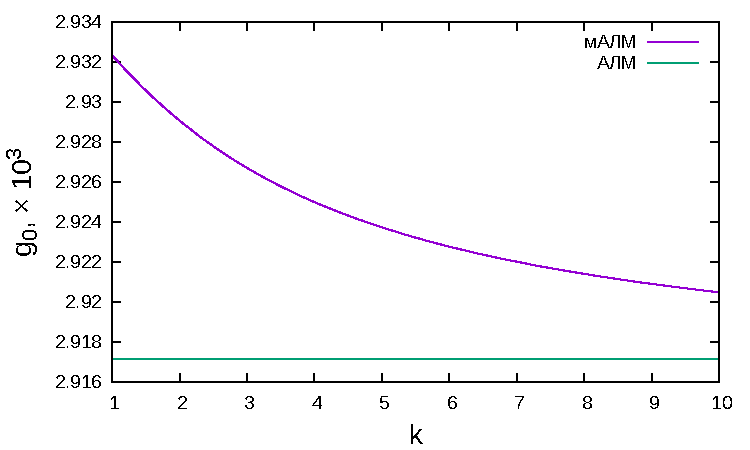
\includegraphics[width=\textwidth]{figs/levmar/convergence/convergence_10.txt_g.pdf}
    \caption{$g_0$}
  \end{subfigure}%
  \begin{subfigure}[b]{0.35\textwidth}
    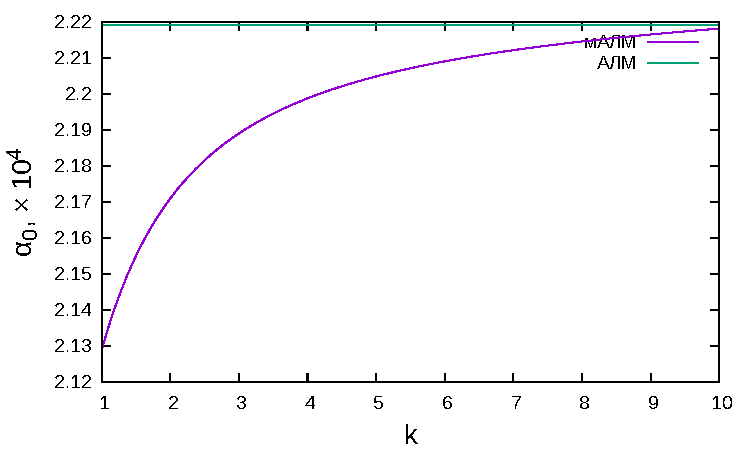
\includegraphics[width=\textwidth]{figs/levmar/convergence/convergence_10.txt_alpha.pdf}
    \caption{$\alpha_0$}
  \end{subfigure}%
  \begin{subfigure}[b]{0.35\textwidth}
    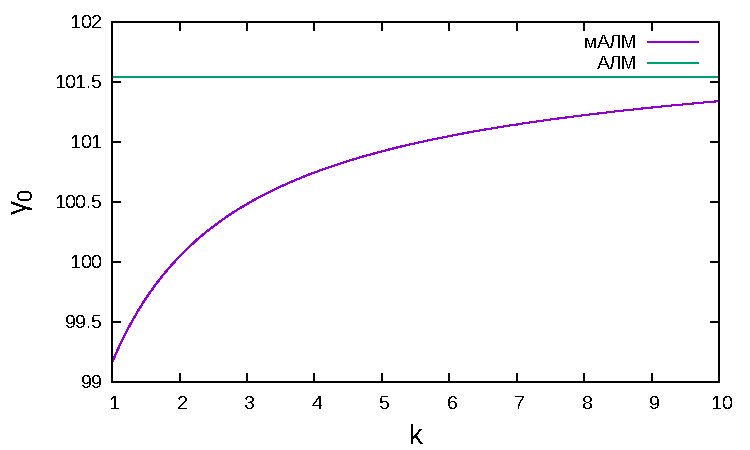
\includegraphics[width=\textwidth]{figs/levmar/convergence/convergence_10.txt_gamma.pdf}
    \caption{$\gamma$}
  \end{subfigure}
  \caption{Зависимость оптимальных параметров от $\sigma_y = 0.02ky, k \in [1; 10]$.}
  \label{fig:conv_10_g}
\end{figure}

\begin{figure}[h]
  \centering
  \begin{subfigure}[b]{0.33\textwidth}
    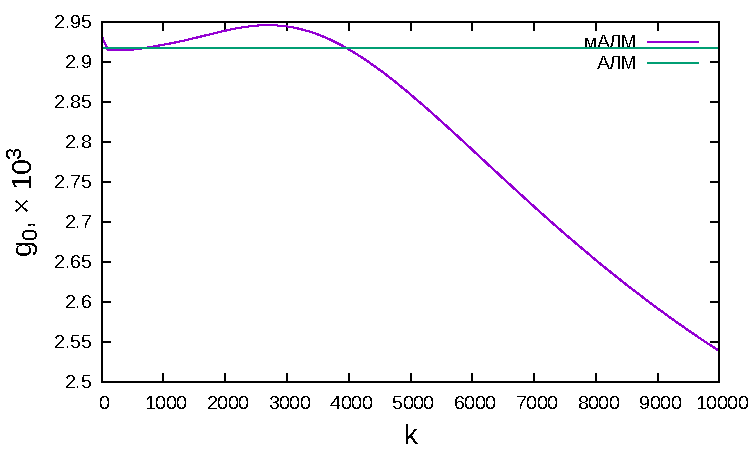
\includegraphics[width=\textwidth]{figs/levmar/convergence/convergence_10000.txt_g.pdf}
    \caption{$g_0$}
  \end{subfigure}%
  \begin{subfigure}[b]{0.33\textwidth}
    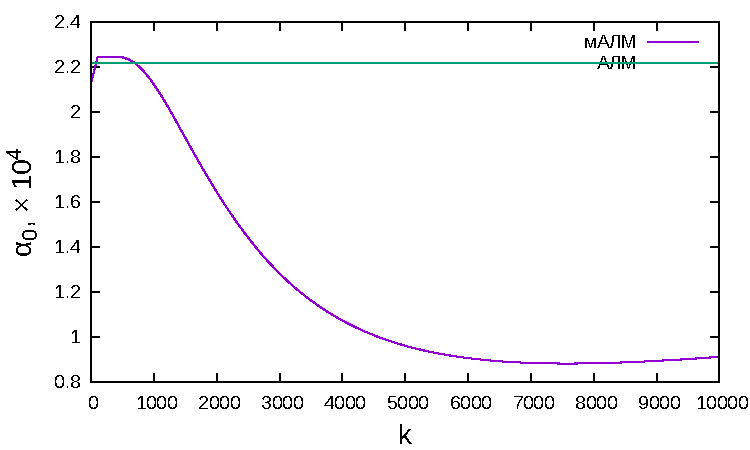
\includegraphics[width=\textwidth]{figs/levmar/convergence/convergence_10000.txt_alpha.pdf}
    \caption{$\alpha_0$}
  \end{subfigure}%
  \begin{subfigure}[b]{0.33\textwidth}
    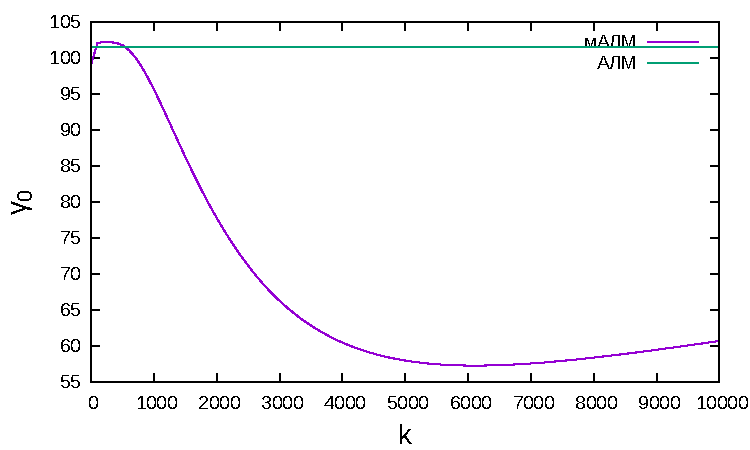
\includegraphics[width=\textwidth]{figs/levmar/convergence/convergence_10000.txt_gamma.pdf}
    \caption{$\gamma$}
  \end{subfigure}
  \caption{Зависимость оптимальных параметров от $\sigma_y = 0.02ky, k \in [1; 10000]$.}
  \label{fig:conv_10000_g}
\end{figure}
\end{comment}

\begin{figure}[h]
  \centering
  \begin{subfigure}[b]{0.5\textwidth}
    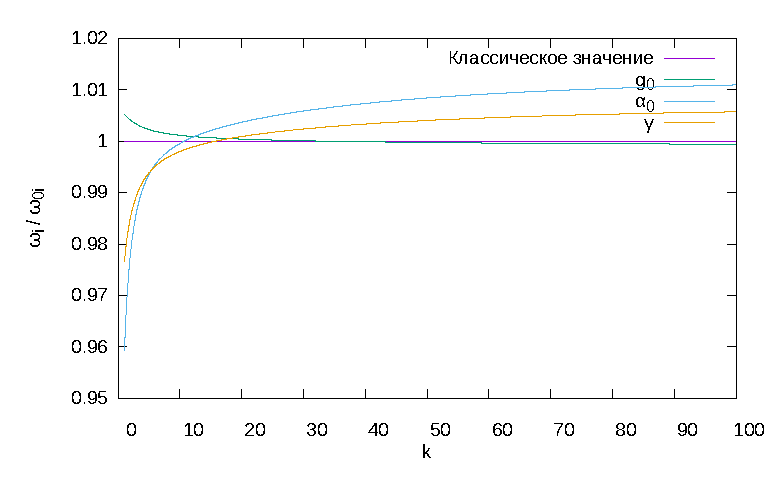
\includegraphics[width=\textwidth]{figs/levmar/convergence/convergence_100.txt.eps}
	\caption{$k \in [1; 100]$}
	\label{fig:conv_100}
  \end{subfigure}%
  \begin{subfigure}[b]{0.5\textwidth}
    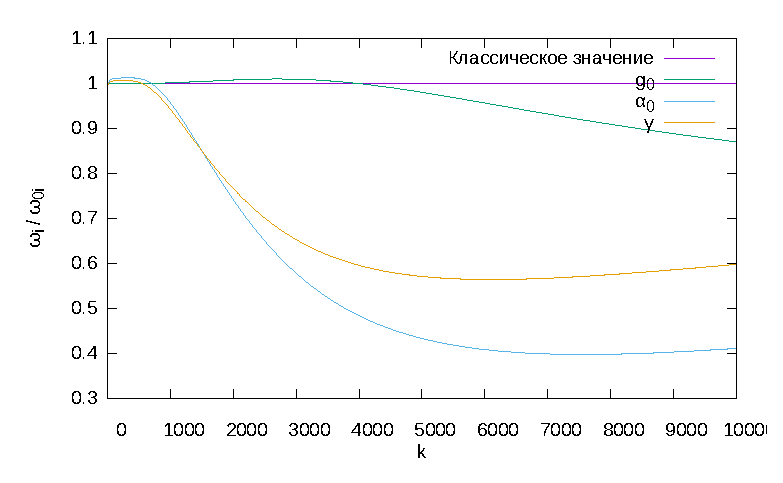
\includegraphics[width=\textwidth]{figs/levmar/convergence/convergence_10000.txt.eps}
	\caption{$k \in [10; 10000]$}
	\label{fig:conv_10000}
  \end{subfigure}
  \caption{Зависимость оптимальных параметров от $\sigma_y = 0.02ky$.}
  \label{fig:conv}
\end{figure}

\FloatBarrier

\bibliographystyle{babunsrt-lf}
%\bibliographystyle{babunsrt}
%\bibliographystyle{unsrt}
\bibliography{bibliography}

\end{document}
